\documentclass[12pt, a4paper]{article}
\usepackage[utf8]{inputenc}
\usepackage{graphicx}
\usepackage{gensymb}
\usepackage{amsmath}
\usepackage{float}
%\usepackage[figurename=Graf]{caption}
\usepackage{subcaption}
\usepackage{caption}

\title{Machine learning}
\author{Miha Pompe}
\date{March 2022}

\begin{document}
\begin{titlepage}
	\centering
 	
\includegraphics[width=0.45\textwidth]{logo_fmf_uni-lj_sl_veliki.png}\par\vspace{1cm}
	\vspace{1cm}
	\vspace{1.5cm}
	{\huge\bfseries Machine learning\par}
	\vspace{2cm}
	{\Large Miha Pompe 28191072\par}
	\vfill
	\vfill
	{\large March 2022\par}
\end{titlepage}
% \maketitle
\thispagestyle{empty}
\clearpage
\pagenumbering{arabic}
\newpage


\section{Introduction}
There are three basic types of machine learning:
\begin{itemize}
  \item Supervised learning
      \begin{itemize}
        \item Classification: sorting into different categories
        \item Regression: modelling or fitting
      \end{itemize}
  \item Unsupervised learning
  \item Stimulated learning
\end{itemize}
In physics we usually deal with the first type, we either want to identify new phenomena or we want to extract a prediction. Machine learning algorithms have the advantage over classical approaches that they can efficiently break down complex problems into simple elements.

Let's describe machine learning more formally. Let there be a set of examples $D = \{(x_k,y_k)\}_{k=1,..,N}$, where $x_k = (x_k^1, ..., x_k^M)$ is a vector of characteristics of size $M$ and $y_k = (y_k^1, ..., y_k^Q)$ is a vector of end results. The aim of a machine learning algorithm is to extract the function $h$, which minimizes the loss function
\begin{equation}
  L(h) = E[L(y, h(x))] = \frac{1}{N}\sum_{k=1}^N L(y_k, h(x_k)).
\end{equation}
$L(\dot,\dot)$ is a function that describes the quality of the prediction, where the values $(x,y)$  and randomly samples from the set $D$. After learning we are left with a function $h(x)$ which given an input set $x$ will produce a prediction $h(x)$. This prediction best fits the initial set of values.

The function $h$ is a combination of many simpler functions with a few free parameters. The ML algorithm tries to adjust those parameters to minimize the loss function.

The function $h$ is described by the following function
\begin{equation}
  h_{w,b}(x) = \theta(w_i x_i + b),
\end{equation}
where $w_i$ is a vector of weights, $b$ is the bias and $\theta$ is a nonlinear function.

The basic building block of a decision tree is a step function $H(x_i-t_i) = 0, 1$ which is equal to 1 for $x_i > t_i$  and 0 otherwise. Here the function $h$ is described as
\begin{equation}
  h(x) = \sum_{i=1}^J a_i H(x_i-t_i).
\end{equation}

We will be testing both methods on a HIGGS dataset, where we will try to differentiate the signal from background.


\section{Analysis of the neural network method}
We constructed a neural network using the Tensorflow framework. Every neural network can be controlled by the following parameters: number of epochs, batch size and the topology of the neural network. The default parameters are: number of epochs is 10, batch size is 1000 and the network will consist of 2 layers each with 50 nodes. In this chapter we will examine the effect of each parameter and determine the optimal neural network.

The success of a neural network can be characterized using three different methods. The first one is the accuracy of prediction when testing a new dataset. The second is the value of the loss function for a new dataset. The third is the area under the ROC curve (AUC). A receiver operating characteristic curve, or ROC curve, is a graphical plot that illustrates the diagnostic ability of a binary classifier system as its discrimination threshold is varied. The ROC curve is created by plotting the true positive rate (TPR) against the false positive rate (FPR) at various threshold settings. Higher accuracy, lower loss value and higher AUC value are all characteristic for successful neural networks. All three show a similar result therefore I've chosen to mostly present the AUC value.

First let's analyze the effect of the number of epochs. The number of epochs is a hyperparameter that defines the number times that the learning algorithm will work through the entire training dataset. The figure 1a shows the accuracy of the model that has been trained with a certain number of epochs. The blue line shows how the model performed on new data, which means this shows a realistic value of accuracy. The orange line shows the accuracy of the model evaluated on training data. We can see here that the accuracy rises with epochs as the model slowly becomes overfitted. In figure 1b we are also looking at the effects of epoch number but here we are looking at the AUC number. A distinct peak can be seen at around 100 epochs, meaning this is the optimal value for achieving the best characterization.

The batch size is a hyperparameter that defines the number of samples to work through before updating the internal model parameters. Figure 1c shows how the AUC value changes with batch size. A peak can be observed at the batch size of 500, where the AUC value reaches 0,74. After that the curve quickly drops.

\begin{figure}[H]
  \begin{subfigure}{0.5\textwidth}
  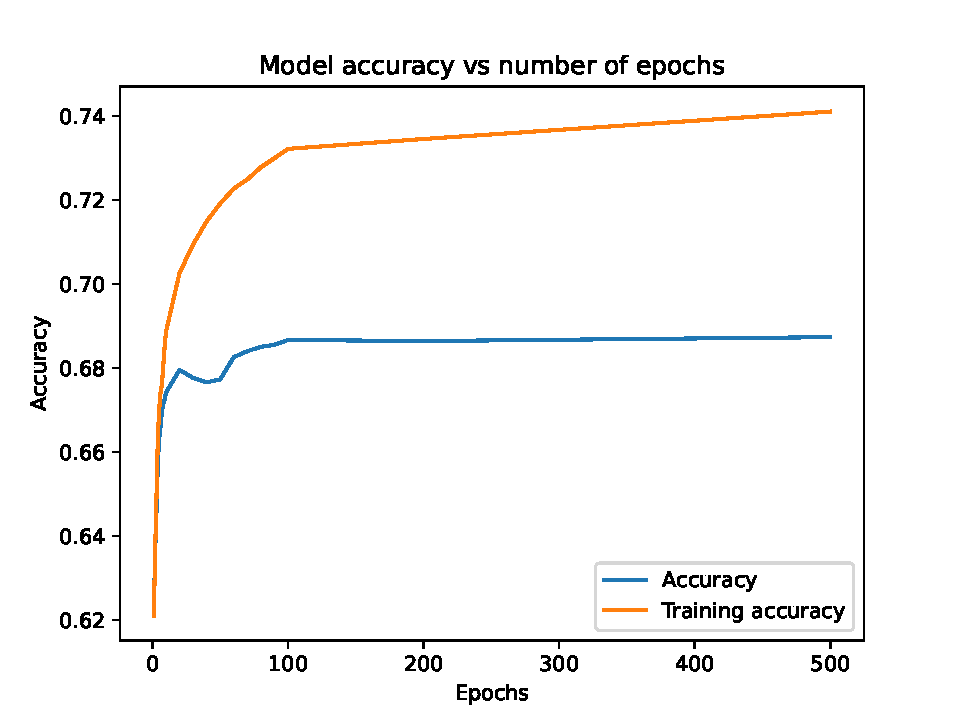
\includegraphics[width=\linewidth]{../graphs/epochs_accuracy.pdf}
  \caption{Model accuracy in comparison with the number of epochs} \label{fig:a}
  \end{subfigure}
  \hspace*{\fill}
  \begin{subfigure}{0.5\textwidth}
  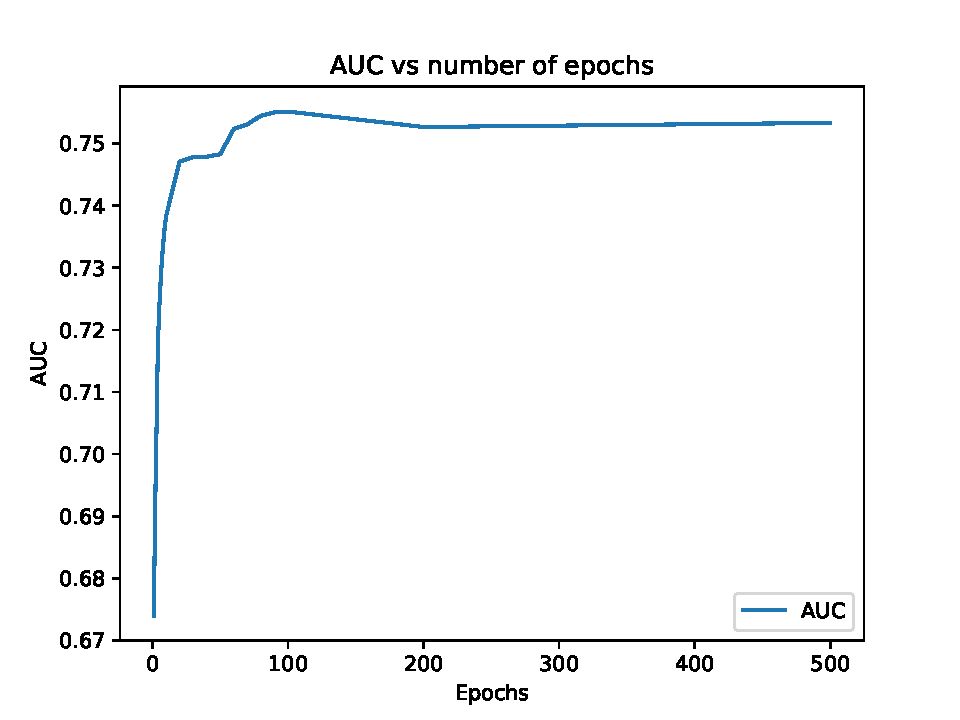
\includegraphics[width=\linewidth]{../graphs/epochs_auc.pdf}
  \caption{AUC number in comparison with the number of epochs} \label{fig:b}
  \end{subfigure}
  \medskip
  \begin{subfigure}{0.5\textwidth}
  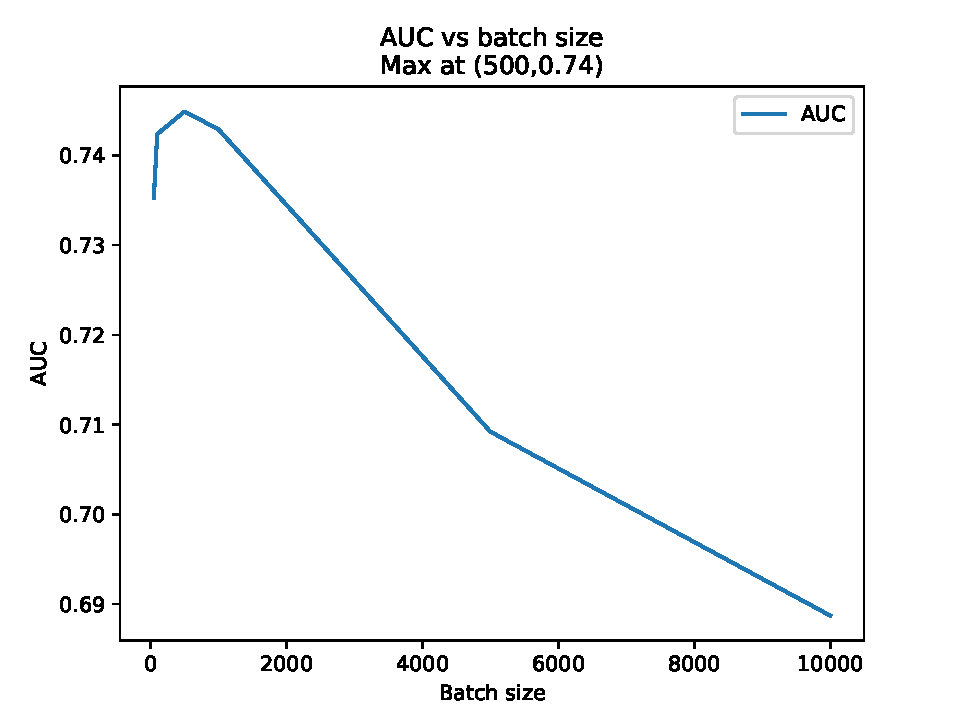
\includegraphics[width=\linewidth]{../graphs/batch_auc.pdf}
  \caption{AUC number in comparison with batch size} \label{fig:c}
  \end{subfigure}
  \hspace*{\fill}
  \begin{subfigure}{0.5\textwidth}
  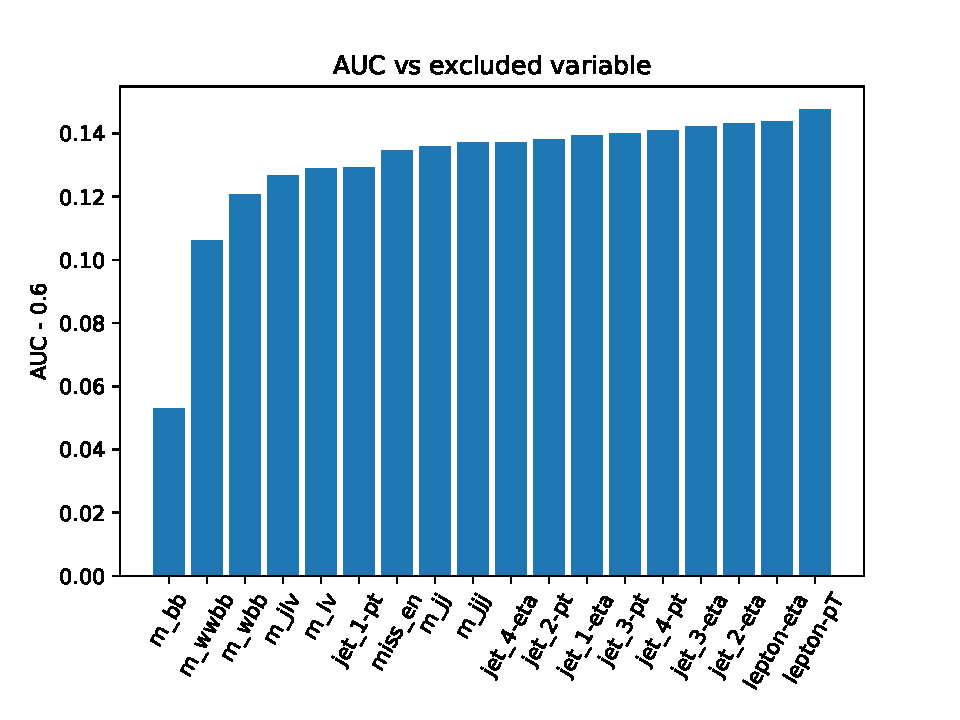
\includegraphics[width=\linewidth]{../graphs/excluded_variable_auc.pdf}
  \caption{AUC number of a model which has been trained by excluding a certain variable} \label{fig:d}
  \end{subfigure} 
  \medskip
  \begin{subfigure}{0.5\textwidth}
  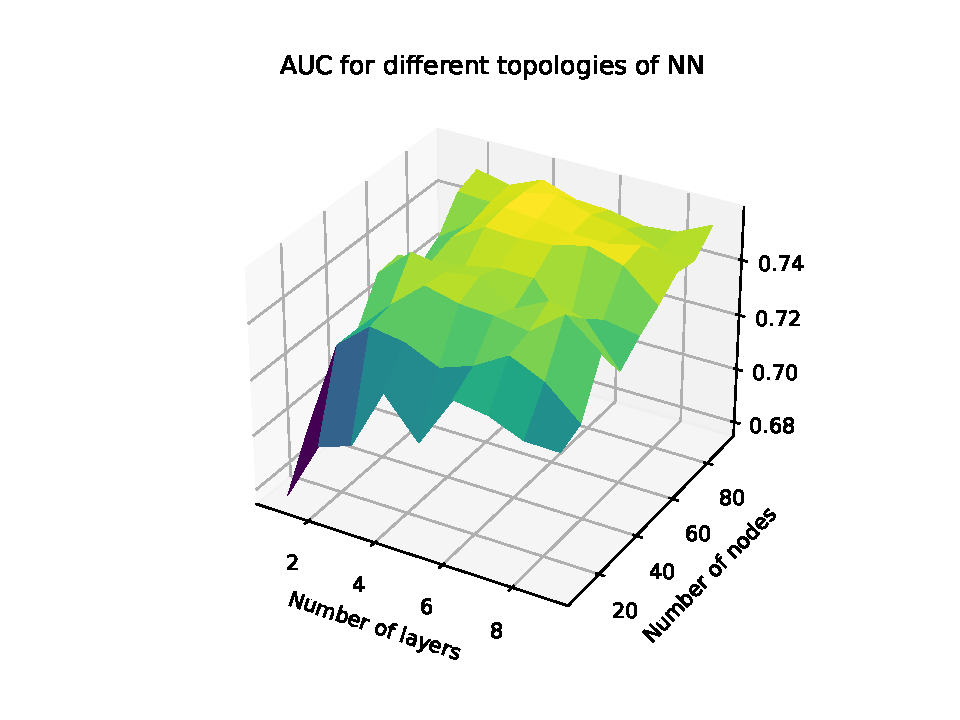
\includegraphics[width=\linewidth]{../graphs/layers_nodes_auc.pdf}
  \caption{AUC number for different topologies of neural networks} \label{fig:c}
  \end{subfigure}
  \hspace*{\fill}
  \begin{subfigure}{0.5\textwidth}
  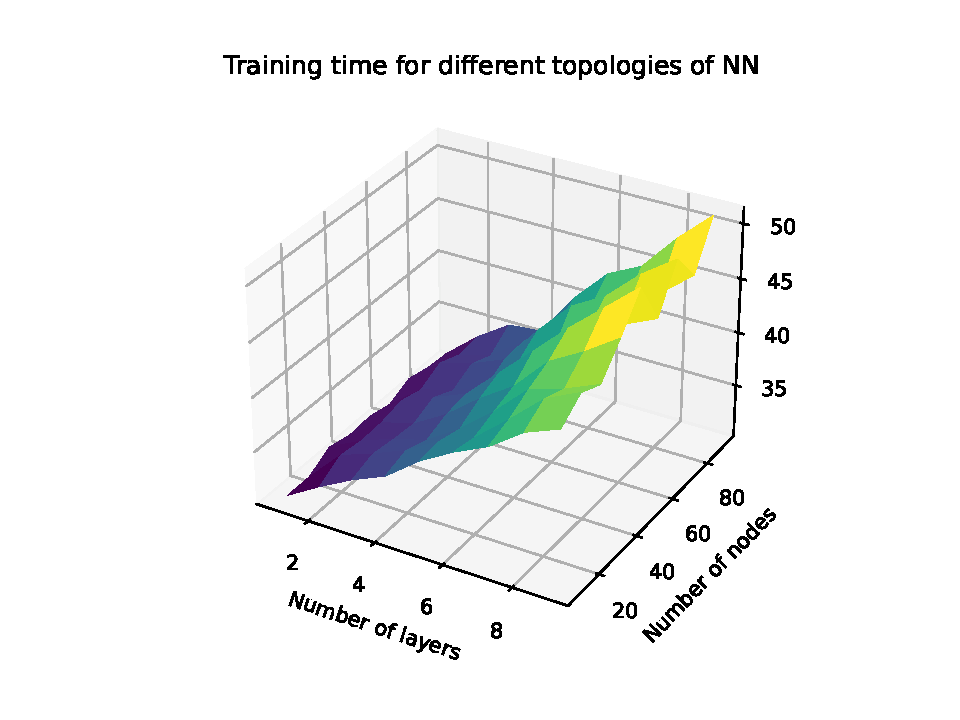
\includegraphics[width=\linewidth]{../graphs/layers_nodes_time.pdf}
  \caption{Training time for different topologies of neural networks} \label{fig:d}
  \end{subfigure} 
  \caption{Neural network testing} \label{fig:1}
\end{figure}

Sometimes not all parameters are relevant to accurately discriminate against end results. Figure 1d shows how the AUC value changes if we omit one variable. The y-axis is shifted by 0,6 in order to better observe the differences. If the AUC value drops significantly after exclusion of a certain variable we can conclude that that variable is important for the success of the model. This happened with variables $m_{bb}$ and $m_{wwbb}$. Most other variables don't greatly affect the model's success.

A very important factor is the shape of the neural network. Figure 1e shows the AUC of neural networks with different number of layers and nodes pre layer. Here all layers have the same number of nodes. We can see that for smaller and simpler neural networks don't perform very well, but as we increase the number of layers and nodes the AUC value reaches a plateau. By adding more layers and nodes we also increase the training time as can be seen in figure 1f. Training time rises linearly both with the number of layers and number of nodes.

\begin{figure}[h!]
  \begin{subfigure}{0.5\textwidth}
  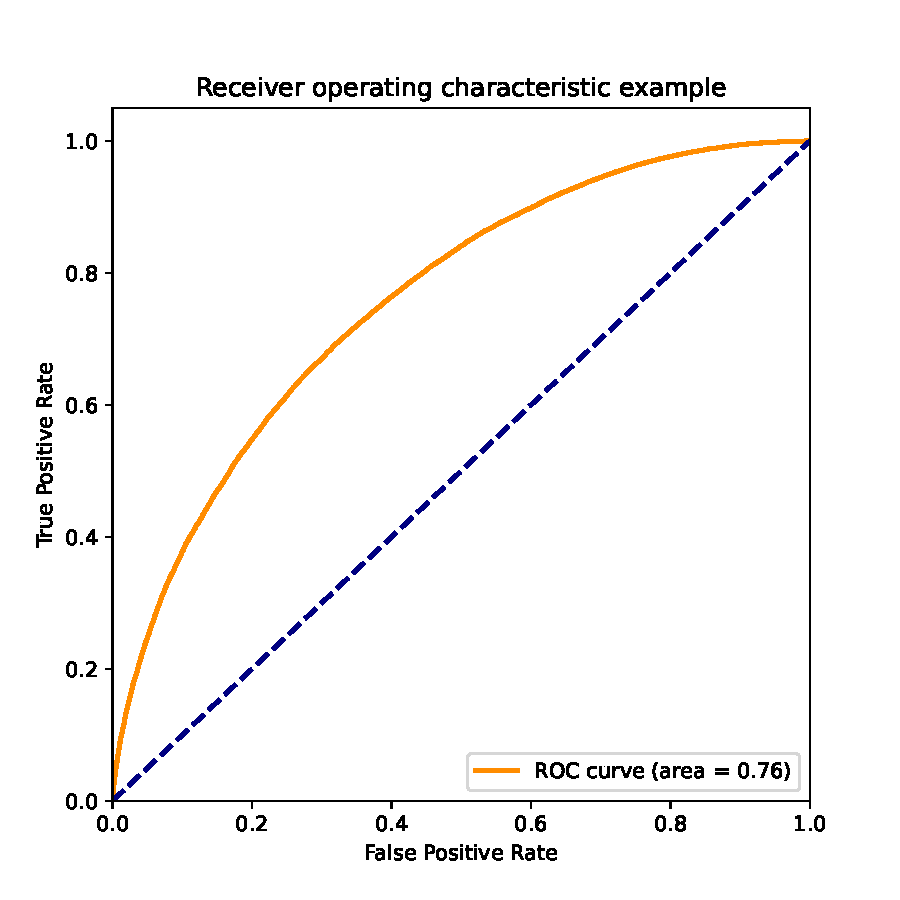
\includegraphics[width=\linewidth]{../graphs/roc-curve.pdf}
  \caption{Receiver operating characteristic curve} \label{fig:a}
  \end{subfigure}
  \hspace*{\fill}
  \begin{subfigure}{0.5\textwidth}
  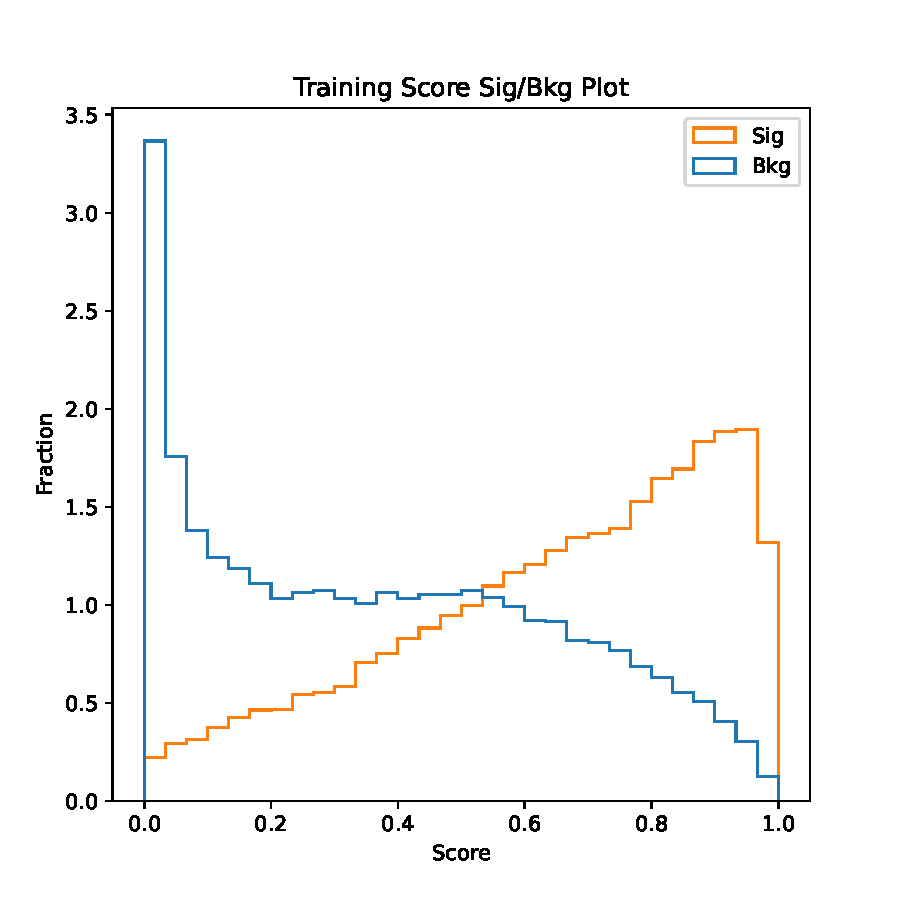
\includegraphics[width=\linewidth]{../graphs/ml-score.pdf}
  \caption{Training score for signal and background} \label{fig:b}
  \end{subfigure}
  \caption{Characteristics of the optimal neural network} \label{fig:1}
\end{figure}

By combining all observations we can determine the optimal neural network. Its parameters are: epoch 100, batch size 500, 7 layers and 60 nodes. Figure 2a shows the ROC curve for this configuration and the AUC is 0,76. This might not be the theoretical maximum as we could also test different shapes of neural networks, not just square ones. Figure 2b shows the training score of the signal and background. 

\section{Analysis of the decision tree method}
The decision tree method is sometimes a good alternative to neural networks. In this section we will see how good it performs on our problem and how it compares with neural networks.

The most important factor with decision trees is the number of estimators. Figure 3a shows how the score of the model (the score is similar to the accuracy we discussed earlier) depends on the number of estimators. We can see a peak at 50 estimators with new data. The score continually increases for the training data. A similar peak can be seen on figure 3b, which show the AUC value in comparison with the number of estimators.

The decision tree method reached a peat at around 0,66 AUC which is far lower compared to neural network's 0,76. We can conclude that the neural networks are better suited for solving this particular problem.

\begin{figure}[h!]
  \begin{subfigure}{0.5\textwidth}
  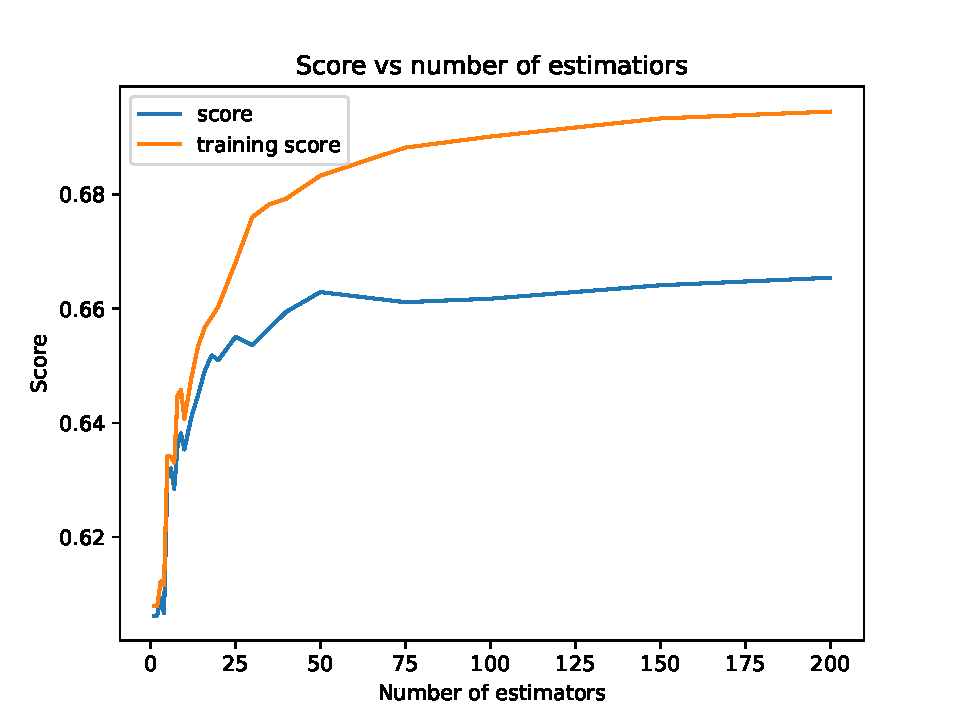
\includegraphics[width=\linewidth]{../graphs/bdt_score_estimators.pdf}
  \caption{Score in comparison with the number of estimators} \label{fig:a}
  \end{subfigure}
  \hspace*{\fill}
  \begin{subfigure}{0.5\textwidth}
  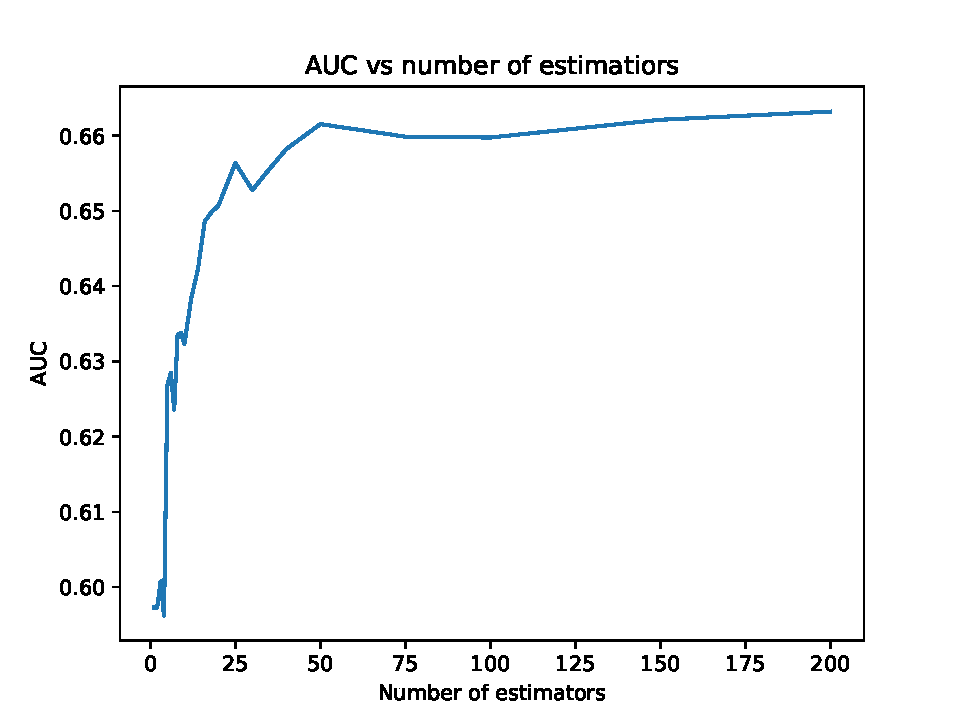
\includegraphics[width=\linewidth]{../graphs/bdt_auc_estimators.pdf}
  \caption{AUC score in comparison with the number of estimators} \label{fig:b}
  \end{subfigure}
  \caption{Decision tree testing} \label{fig:1}
\end{figure}

\end{document}